% Construction : deux états A en (0,0) et B en (3.4,0), rayon 0.55.
%   Arcs A→B de poids a, B→A de poids b, boucles A→A de 1−a et B→B de 1−b.
% SVG : x = 60 + 46x, y = 90.
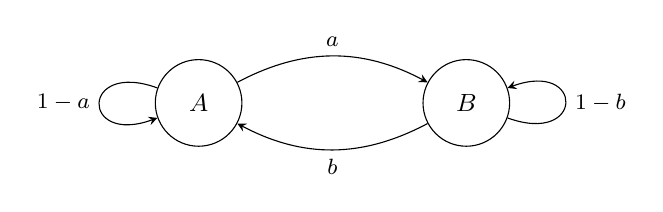
\begin{tikzpicture}[scale=1, >=stealth, every node/.style={font=\small}]
  \node[draw, circle, minimum size=11mm] (A) at (0,0) {$A$};
  \node[draw, circle, minimum size=11mm] (B) at (3.4,0) {$B$};
  \draw[->] (A) to[bend left=28] node[above, font=\footnotesize] {$a$} (B);
  \draw[->] (B) to[bend left=28] node[below, font=\footnotesize] {$b$} (A);
  \draw[->] (A) to[out=160, in=200, looseness=7] node[left, font=\footnotesize] {$1-a$} (A);
  \draw[->] (B) to[out=-20, in=20, looseness=7] node[right, font=\footnotesize] {$1-b$} (B);
\end{tikzpicture}
